
\item From point \( A \) located on a highway (Fig. 1.2) one has to get by car as soon as possible to point \( B \) located in the field at a distance \( l \) from the highway. It is known that the car moves in the field \( \eta \) times slower than on the highway. At what distance from point \( D \) one must turn off the highway?
    \begin{center}
        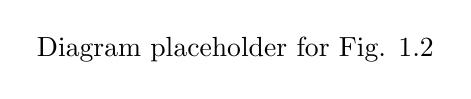
\begin{tikzpicture}
            \node at (0, 0) {Diagram placeholder for Fig. 1.2};
            % The actual TikZ commands for the diagram should go here
        \end{tikzpicture}
    \end{center}
    % Since there are no subquestions in the text provided, I am not including an enumerate environment. Should there be subquestions, the following template can be used:
    % \begin{enumerate}
    %     \item This is a subquestion.
    %     \item This is another subquestion.
    % \end{enumerate}
\begin{solution}
    \begin{center}
        \begin{tikzpicture}
            \pic at (0, 0) {frame=3cm};
        \end{tikzpicture}
    \end{center}
    
    \begin{align*}
        \intertext{Let the car turns off the highway at a distance \( x \) from the point \( D \). So, \( CD = x \), and if the speed of the car in the field is \( v \), then the time taken by the car to cover the distance \( AC = (AD - x) \) on the highway}
        t_1 &= \dfrac{AD - x}{\eta v} \tag{1}\\
        \intertext{and the time taken to travel the distance \( CB \) in the field}
        t_2 &= \dfrac{\sqrt{l^2 + x^2}}{v} \tag{2}\\
        \intertext{So, the total time elapsed to move the car from point \( A \) to \( B \)}
        t &= t_1 + t_2 = \dfrac{AD - x}{\eta v} + \dfrac{\sqrt{l^2 + x^2}}{v}\\
        \intertext{For \( t \) to be minimum}
        \dfrac{dt}{dx} &= 0 \text{ or } \dfrac{1}{v} \left[ -\dfrac{1}{\eta} + \dfrac{x}{\sqrt{l^2 + x^2}} \right] = 0\\
        \eta^2 x^2 &= l^2 + x^2 \text{ or } x = \dfrac{l}{\sqrt{\eta^2 - 1}}
    \end{align*}
\end{solution}